% Options for packages loaded elsewhere
\PassOptionsToPackage{unicode}{hyperref}
\PassOptionsToPackage{hyphens}{url}
%
\documentclass[
]{book}
\usepackage{lmodern}
\usepackage{amssymb,amsmath}
\usepackage{ifxetex,ifluatex}
\ifnum 0\ifxetex 1\fi\ifluatex 1\fi=0 % if pdftex
  \usepackage[T1]{fontenc}
  \usepackage[utf8]{inputenc}
  \usepackage{textcomp} % provide euro and other symbols
\else % if luatex or xetex
  \usepackage{unicode-math}
  \defaultfontfeatures{Scale=MatchLowercase}
  \defaultfontfeatures[\rmfamily]{Ligatures=TeX,Scale=1}
\fi
% Use upquote if available, for straight quotes in verbatim environments
\IfFileExists{upquote.sty}{\usepackage{upquote}}{}
\IfFileExists{microtype.sty}{% use microtype if available
  \usepackage[]{microtype}
  \UseMicrotypeSet[protrusion]{basicmath} % disable protrusion for tt fonts
}{}
\makeatletter
\@ifundefined{KOMAClassName}{% if non-KOMA class
  \IfFileExists{parskip.sty}{%
    \usepackage{parskip}
  }{% else
    \setlength{\parindent}{0pt}
    \setlength{\parskip}{6pt plus 2pt minus 1pt}}
}{% if KOMA class
  \KOMAoptions{parskip=half}}
\makeatother
\usepackage{xcolor}
\IfFileExists{xurl.sty}{\usepackage{xurl}}{} % add URL line breaks if available
\IfFileExists{bookmark.sty}{\usepackage{bookmark}}{\usepackage{hyperref}}
\hypersetup{
  pdftitle={Life Contingencies: The Mathematics, Statistics, and Economics of Life Insurance},
  pdfauthor={An open text authored by the Actuarial Community},
  hidelinks,
  pdfcreator={LaTeX via pandoc}}
\urlstyle{same} % disable monospaced font for URLs
\usepackage{longtable,booktabs}
% Correct order of tables after \paragraph or \subparagraph
\usepackage{etoolbox}
\makeatletter
\patchcmd\longtable{\par}{\if@noskipsec\mbox{}\fi\par}{}{}
\makeatother
% Allow footnotes in longtable head/foot
\IfFileExists{footnotehyper.sty}{\usepackage{footnotehyper}}{\usepackage{footnote}}
\makesavenoteenv{longtable}
\usepackage{graphicx,grffile}
\makeatletter
\def\maxwidth{\ifdim\Gin@nat@width>\linewidth\linewidth\else\Gin@nat@width\fi}
\def\maxheight{\ifdim\Gin@nat@height>\textheight\textheight\else\Gin@nat@height\fi}
\makeatother
% Scale images if necessary, so that they will not overflow the page
% margins by default, and it is still possible to overwrite the defaults
% using explicit options in \includegraphics[width, height, ...]{}
\setkeys{Gin}{width=\maxwidth,height=\maxheight,keepaspectratio}
% Set default figure placement to htbp
\makeatletter
\def\fps@figure{htbp}
\makeatother
\setlength{\emergencystretch}{3em} % prevent overfull lines
\providecommand{\tightlist}{%
  \setlength{\itemsep}{0pt}\setlength{\parskip}{0pt}}
\setcounter{secnumdepth}{5}
\usepackage{booktabs}
\usepackage{pdfpages}
\setcounter{secnumdepth}{2}
\let\oldmaketitle\maketitle
\AtBeginDocument{\let\maketitle\relax}
\usepackage[]{natbib}
\bibliographystyle{econPeriod}

\title{Life Contingencies: The Mathematics, Statistics, and Economics of Life Insurance}
\author{An open text authored by the Actuarial Community}
\date{}

\begin{document}
\maketitle

\thispagestyle{empty}
%\begin{center}
%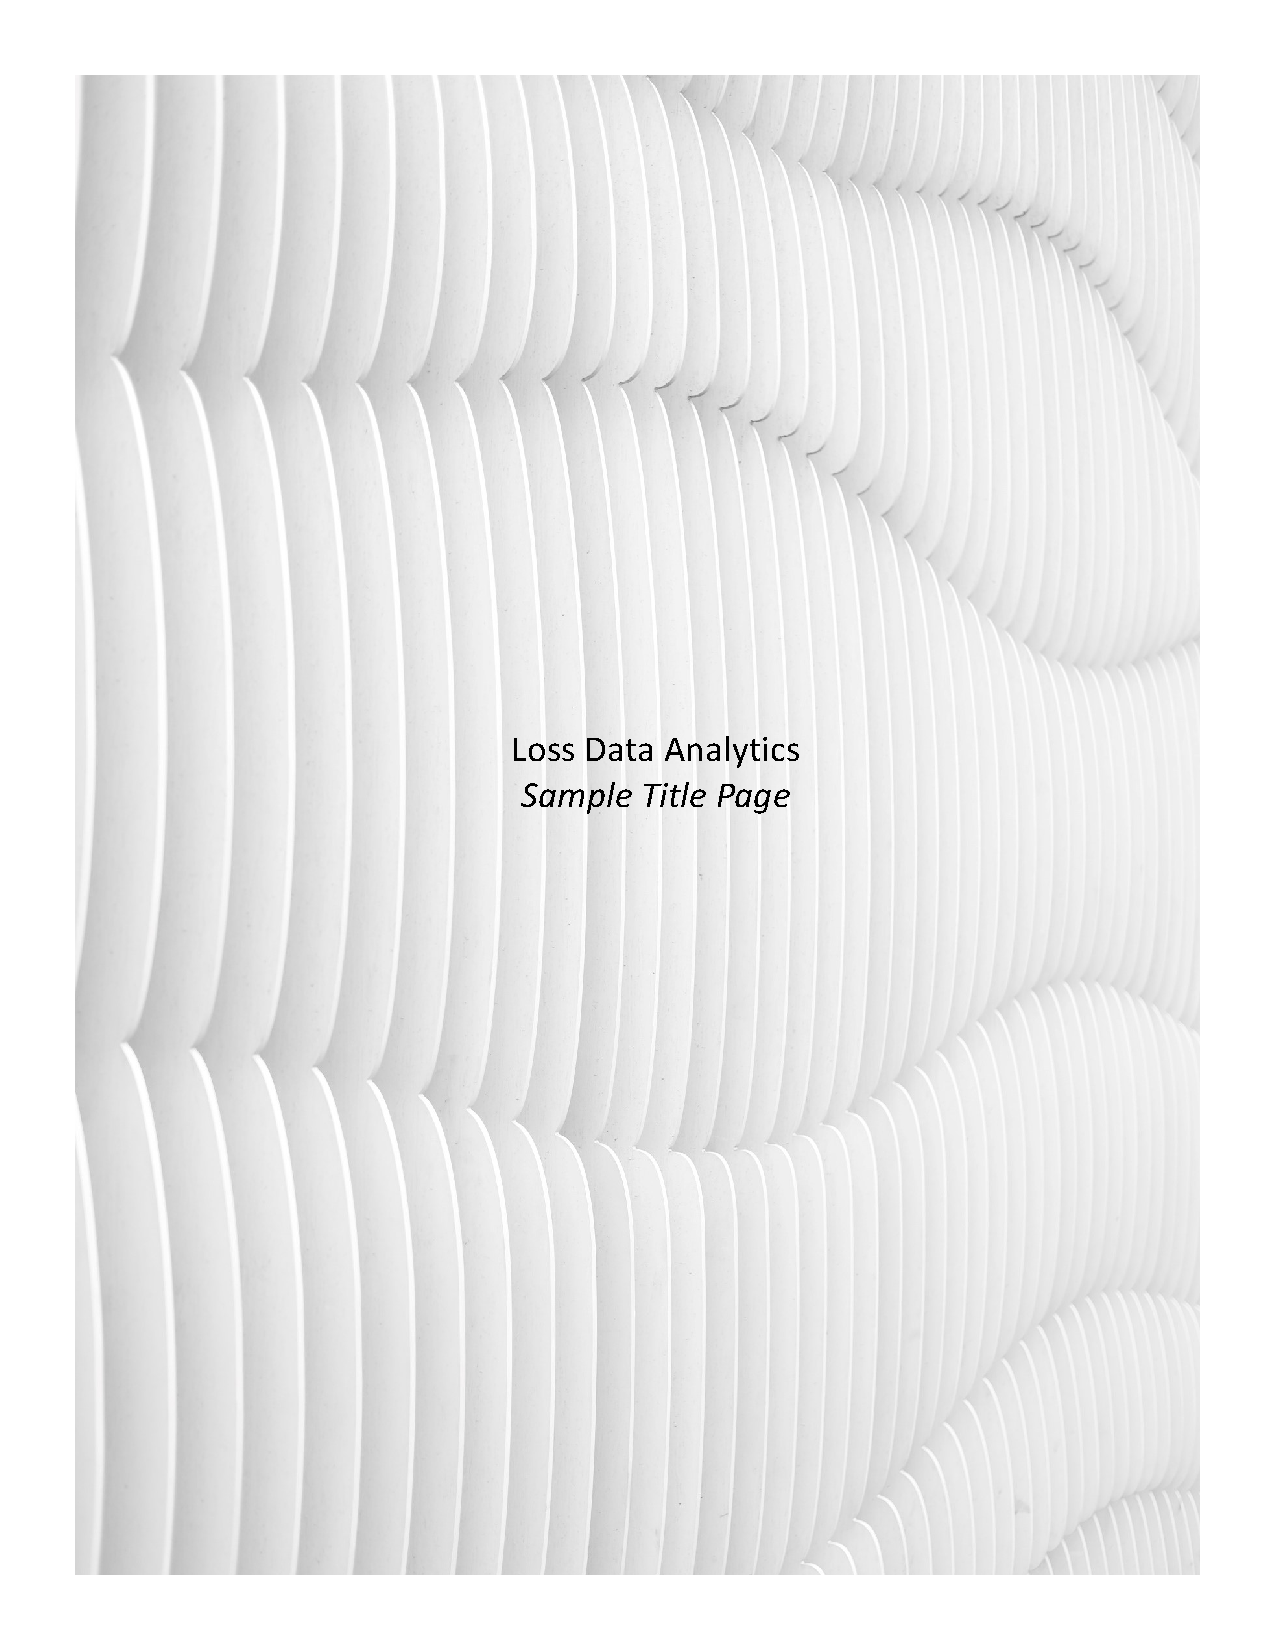
\includepdf{title.pdf}
%\end{center}

\let\maketitle\oldmaketitle
\maketitle

{
\setcounter{tocdepth}{2}
\tableofcontents
}
\hypertarget{preface}{%
\chapter*{Preface}\label{preface}}
\addcontentsline{toc}{chapter}{Preface}

\emph{Date: 17 June 2021}

\hypertarget{book-description}{%
\subsubsection*{Book Description}\label{book-description}}
\addcontentsline{toc}{subsubsection}{Book Description}

\hypertarget{how-will-the-text-be-used}{%
\subsubsection*{How will the text be used?}\label{how-will-the-text-be-used}}
\addcontentsline{toc}{subsubsection}{How will the text be used?}

\hypertarget{why-is-this-good-for-the-profession}{%
\subsubsection*{Why is this good for the profession?}\label{why-is-this-good-for-the-profession}}
\addcontentsline{toc}{subsubsection}{Why is this good for the profession?}

\hypertarget{life-contingent-calculations}{%
\subsubsection*{Life Contingent Calculations}\label{life-contingent-calculations}}
\addcontentsline{toc}{subsubsection}{Life Contingent Calculations}

\hypertarget{project-goal}{%
\subsubsection*{Project Goal}\label{project-goal}}
\addcontentsline{toc}{subsubsection}{Project Goal}

\hypertarget{acknowledgements}{%
\section*{Acknowledgements}\label{acknowledgements}}
\addcontentsline{toc}{section}{Acknowledgements}

\hypertarget{contributors}{%
\section*{Contributors}\label{contributors}}
\addcontentsline{toc}{section}{Contributors}

\hypertarget{for-our-readers}{%
\section*{For our Readers}\label{for-our-readers}}
\addcontentsline{toc}{section}{For our Readers}

\hypertarget{introduction}{%
\chapter{Introduction}\label{introduction}}

Placeholder

\hypertarget{S:MortData}{%
\section{Mortality data: Life Expectancies, Deaths, Counts, \& Features}\label{S:MortData}}

\hypertarget{life-expectancies}{%
\subsection{Life Expectancies}\label{life-expectancies}}

\hypertarget{population-mortality-counts}{%
\subsection{Population Mortality Counts}\label{population-mortality-counts}}

\hypertarget{S:IndivMortData}{%
\subsection{Individual Mortality Data}\label{S:IndivMortData}}

\hypertarget{Sec:ModelingDeaths}{%
\section{Modeling Death}\label{Sec:ModelingDeaths}}

\hypertarget{lifetime-random-variable-and-its-distribution}{%
\subsection{Lifetime random variable and its distribution}\label{lifetime-random-variable-and-its-distribution}}

\hypertarget{survival-and-mortality-probabilities}{%
\subsection{Survival and mortality probabilities}\label{survival-and-mortality-probabilities}}

\hypertarget{S:LifeExp}{%
\subsection{Complete expectation of life}\label{S:LifeExp}}

\hypertarget{S:AnalMortLaws}{%
\section{Analytical laws of mortality}\label{S:AnalMortLaws}}

\hypertarget{S:LifeTab}{%
\section{Life tables and their functions}\label{S:LifeTab}}

\hypertarget{S:LifeTabBasic}{%
\subsection{Life table based on U.S. population data}\label{S:LifeTabBasic}}

\hypertarget{S:LifeTabMImpr}{%
\subsection{Mortality Improvement Modeling}\label{S:LifeTabMImpr}}

\hypertarget{S:NonParamSurv}{%
\section{Non-parametric survival estimation}\label{S:NonParamSurv}}

\hypertarget{Sec:LifeTableRecursive}{%
\section{Appendix 2A. Life Table: Recursive Calculations}\label{Sec:LifeTableRecursive}}

\hypertarget{C:SimpleBenefit}{%
\chapter{Basic Life Contingent Benefits}\label{C:SimpleBenefit}}

Placeholder

\hypertarget{Sec:BenefitCFunc}{%
\section{Valuation of cash flows under uncertainty}\label{Sec:BenefitCFunc}}

\hypertarget{moment-calculations}{%
\subsection{Moment Calculations}\label{moment-calculations}}

\hypertarget{illustrative-moments-of-cash-flows}{%
\subsection{Illustrative Moments of Cash Flows}\label{illustrative-moments-of-cash-flows}}

\hypertarget{Sec:BenefitActNot}{%
\section{Life insurance benefits}\label{Sec:BenefitActNot}}

\hypertarget{Sec:BenefitWL}{%
\subsection{Whole of life insurance}\label{Sec:BenefitWL}}

\hypertarget{Sec:BenefitTI}{%
\subsection{Term insurance}\label{Sec:BenefitTI}}

\hypertarget{pure-endowment}{%
\subsection{Pure endowment}\label{pure-endowment}}

\hypertarget{endowment-insurance}{%
\subsection{Endowment insurance}\label{endowment-insurance}}

\hypertarget{Sec:BenefitAnnuity}{%
\section{Life annuity benefits}\label{Sec:BenefitAnnuity}}

\hypertarget{life-annuity}{%
\subsection{Life annuity}\label{life-annuity}}

\hypertarget{term-life-annuity}{%
\subsection{Term life annuity}\label{term-life-annuity}}

\hypertarget{deferred-life-annuity}{%
\subsection{Deferred life annuity}\label{deferred-life-annuity}}

\hypertarget{guaranteed-life-annuity}{%
\subsection{Guaranteed life annuity}\label{guaranteed-life-annuity}}

\hypertarget{Sec:BenefitCS}{%
\section{Case Study: A portfolio of term insurance policies}\label{Sec:BenefitCS}}

\hypertarget{Sec:BenefitCSInd}{%
\subsection{An individual policy}\label{Sec:BenefitCSInd}}

\hypertarget{further-resources-and-contributors}{%
\section{Further Resources and Contributors}\label{further-resources-and-contributors}}

\hypertarget{contributors-1}{%
\subsubsection*{Contributors}\label{contributors-1}}
\addcontentsline{toc}{subsubsection}{Contributors}

\hypertarget{Sec:ExamplesValCash}{%
\section{Appendix 3A. Examples of valuation of general cash flows}\label{Sec:ExamplesValCash}}

\hypertarget{example-3.1.1.-varying-payments-and-rates-of-interest}{%
\subsubsection*{Example 3.1.1. Varying Payments and Rates of Interest}\label{example-3.1.1.-varying-payments-and-rates-of-interest}}
\addcontentsline{toc}{subsubsection}{Example 3.1.1. Varying Payments and Rates of Interest}

\hypertarget{example-3.1.2.-varying-payments-and-rates-of-interest-with-uncertainty}{%
\subsubsection*{Example 3.1.2. Varying Payments and Rates of Interest With Uncertainty}\label{example-3.1.2.-varying-payments-and-rates-of-interest-with-uncertainty}}
\addcontentsline{toc}{subsubsection}{Example 3.1.2. Varying Payments and Rates of Interest With Uncertainty}

\hypertarget{C:BenefitExt}{%
\chapter{Extensions to Modeling Basic Life Contingent Benefits}\label{C:BenefitExt}}

Placeholder

\hypertarget{the-impact-of-self-selection}{%
\section{The impact of self selection}\label{the-impact-of-self-selection}}

\hypertarget{modelling-contingent-cash-flows-more-frequently-than-annually}{%
\section{Modelling contingent cash flows more frequently than annually}\label{modelling-contingent-cash-flows-more-frequently-than-annually}}

\hypertarget{table-of-contents}{%
\section{Table of Contents}\label{table-of-contents}}

\hypertarget{C:NotationConventionLC}{%
\chapter{Appendix: Conventions for Notation}\label{C:NotationConventionLC}}

Placeholder

\hypertarget{S:NC:ActSymbols}{%
\section{Actuarial Notation}\label{S:NC:ActSymbols}}

\hypertarget{life-table-symbols}{%
\subsection{Life Table Symbols}\label{life-table-symbols}}

\hypertarget{Sec:LifeInsSymbols}{%
\subsection{Life Insurance Symbols}\label{Sec:LifeInsSymbols}}

\hypertarget{Sec:LifeAnnSymbols}{%
\subsection{Annuity Certain and Life Annuity Symbols}\label{Sec:LifeAnnSymbols}}

\hypertarget{C:NotConv:Halo}{%
\section{Halo System}\label{C:NotConv:Halo}}

\hypertarget{S:NC:General}{%
\section{General Conventions}\label{S:NC:General}}

\hypertarget{S:NC:Abbreviations}{%
\section{Abbreviations}\label{S:NC:Abbreviations}}

\hypertarget{S:NC:StatSymbols}{%
\section{Common Statistical Symbols and Operators}\label{S:NC:StatSymbols}}

\hypertarget{S:NC:Symbols}{%
\section{Common Mathematical Symbols and Functions}\label{S:NC:Symbols}}

\hypertarget{further-readings}{%
\section{Further Readings}\label{further-readings}}

Time taken for this draft of the book: 0 minutes.

  \bibliography{References/LDAReference2020A.bib}

\end{document}
